\chapter{Background Theory}
\label{chp:theory} 

\section{Robotic Maintenance of Industrial Installations}

\subsection{Introduction}

This project is a small step towards a larger long-term goal concerning robotic maintenance on topside offshore installations. This section puts the following background theory, and the implementation described in chapter \ref{chp:implementation}, into the context of the long-term goal. 

This section provides a brief introduction to how topside maintenance is performed today, how these maintenance tasks could be robotized. The section is concluded with a discussion on how well modern robotics is suited for the task. 

\subsection{Potential Maintenance Tasks}

Hidden failure modes: PFD: What is the probability that a device (Fire detector, shut down valve, etc.) will fail when needed? 
Solution: Periodic maintenance.

\subsection{Which Tasks Can Be Robotized?}

%In light of the factors listed earlier, maintenance and service robots will be designed with the following goals in mind\cite{AutonomousOG}:

Over the last decade, the \ac{OG} industry has shown an increased interest in the potential benefits of automating the normal operation of remote offshore installations. Some satellite platforms, such as Sleipner B and the more recent Valemon platform are already unmanned during normal operation. It is now clear that robotics has several potential applications in process plants, and particularly in remote \ac{OG} installations. It is, however, difficult to predict how and to what extent robots will be applied in plant automation, as other innovative solutions may arise\cite{statoil_ubemannet}\cite{subsea_konkurranse}\cite{E24}. Current research on plant automation is mainly motivated by two factors\cite{AutonomousOG} \cite{StepwiseApproachToRobotics}:

\begin{itemize}
	\item \textbf{HSE} - Reduced risk exposure for personnel and environment. 
	\item \textbf{Efficiency} - Accomplish more with less effort, resources and time. This means cost reduction by keeping downtime to a minimum with the least amount of effort.
\end{itemize} 

An additional overarching driving factor is that \ac{OG} fields are becoming more difficult to reach. As \ac{OG} fields in shallow waters are depleted, production is moved to deeper waters. This complicates the extraction process and reduces the profit margin. A solution to this challenge is to increase efficiency through further automation. To what extent automation will be in the form of robots, or other innovative solutions is difficult to say. 

\begin{table}
\centering
\begin{tabular}{ |p{2cm} p{3cm} p{5cm}| }
\hline
\multicolumn{3}{|c|}{Robot Applications Including Categorization}\\
\hline\hline
Category & Robot & Robot Task/Activity Description \\ 
\hline
B & Pipeline rigging robot & To autonomously load and offload pigs into pipelines. \\
C & Boat handling robot < 500 kg & To transfer personnel and loads below 500 kg to and from boats.\\
D & Boat handling robot > 500 kg & To transfer loads above 500 kg to and from boats.\\
\hline
B & Mobile universal service robot version 1 & To perform ''buddy'' roles; carrying, holding, lifting, personal safety monitoring etc. \\
C & Mobile universal service robot version 2 & To autonomously perform task not involving manipulation of the process or facilities.\\
D & Mobile universal service robot version 3 & To autonomously perform tasks involving manipulation of the process or facilities. \\
D & Treatment/Inspection robot & To autonomously perform inspection/treatment(painting) tasks of structures/vessels or facilities.\\
\hline
A & Domestic service robot & To autonomously perform floor cleaning, catering, laundry handling, storage handling and logistics activities. \\
\hline\hline 
\end{tabular}
\caption{Some tasks with potential to be ''robotized'', and the corresponding robot category\cite{6094661}.} 
\label{tab:tasks_capabilities}
\end{table}

A feasibility study performed by researchers from \ac{Fraunhofer IPA} identified several topside production tasks and ranked them according to their resource demand. 
%Table \ref{tab:tasks} shows the ranked tasks based on a preselected installation. While all tasks would benefit from ''robotizing'',  
Based on the identified tasks, the study went on to describe a set of specific tasks, and then assess how easy or hard it would be to ''robotize'' these tasks. Table \ref{tab:tasks_capabilities} associates a set of tasks with different robot categories, as well as how easy or hard the process of ''robotizing'' the activity is expected to be. The difficulty levels are described with the letters ''A'' through ''D'', where  ''A'' is described as of the shelf robotics, which makes ''robotizing'' easy. Activities associated with the letter ''D'' on the other hand, cannot be be ''robotized'' with either current or near future technology even if doing so would be beneficial \cite{6094661}. Note that the paper in question is from 2011, and the difficulty of these tasks may have changed. This is particularly true in the domain of visual sensors, given the bloom of 3d sensor technology over the last six years. Some further elaboration on inspection activities and environmental considerations is given in the next subsection. 
%\begin{table}[h!]
%\centering
%\begin{tabular}{ |p{5cm} p{2cm} p{2.5cm} | }
%\hline
% \multicolumn{3}{|c|}{Production Operation Activities} \\
% \hline\hline
% Task & Annual Man Hours & Frequency of Operations\\
% \hline
% Gas compression system operation & 4079    &Daily \\
% Ops checks \& logging & 2350 & Daily\\
% Safety Checks & 1982 & Weekly \\
% Sampling and top-up (glycol, condensate, jet A1)& 1125  & Daily\\
% Chemical Injection \& Handling & 814  & Daily   \\
% Deluge valve system & 819  & Monthly \\
% Supply \& crew boat handling & 568 & Weekly \\
% Materials handling and ordering & 446 & Daily \\
% Helicopter refuelling & 208 & weekly (?) \\
% Helicopter handling & ? & 2 days (daily?) \\
% Sump content clearance & 129 & Weekly \\
% Well testing & 79 & Daily \\
% Diesel/water bunkering & 52 & 2 Weekly \\
% First aid painting & ? & As required \\
% Pigging activities & 40 & Monthly \\
% \hline\hline
%\end{tabular}
%\label{tab:tasks_ranked}
%\caption{Identified and ranked production operation activities \cite{6094661}. Question marks and parenthesis are intentional.} 
%\end{table}

\subsection{Structural Maintenance and Environmental Considerations}

\subsubsection{Corrosion}

Offshore installations are regularly, if not continuously, exposed to harsh weather conditions in the form of wind and seawater. Presence of seawater, either through direct contact or in the form of drops and vapor, forms a very corrosive environment. The offshore and marine environment is classified as the most corrosive environment in ISO 12944\cite{ElReedy2012383}. It is essential to provide countermeasures to ensure safe and reliable operation over the lifetime of the installation. Common corrosion prevention methods are\cite{ElReedy2012383}:

\begin{itemize}
	\item Sacrificial Anodes.
	\item \ac{CP} in the form of a DC-current.
	\item Protective coating.
\end{itemize} 

In terms of maintenance, the sacrificial anodes can be subjected to periodic inspections and replacements, which could be done by a robot. \ac{CP} can more easily be implemented with automated self tests, and should normally not require any inspections and maintenance\cite{ElReedy2012383}. Application of protective coating should ideally be applied in the controlled environment of a workshop. If protective coating is to be applied at sea, one should strive to make the conditions as favorable as possible. 

\subsubsection{Structural Fatigue}

Waves, wind, water currents and other forces subject offshore installations to structural stress. To keep the offshore installations from failing in these conditions, they may be subjected to a \ac{RBI} regime. In brief, \ac{RBI} is a strategy where inspection and maintenance programs are developed based on which risk factors an installation is exposed to. In an automated maintenance program, an autonomous robot could perform inspections of the structure and generate reports based on risk factors such as\cite{ElReedy2012563}:

\begin{description}
\item[Marine growth at sea level] Marine growth will increase the diameter of supporting legs at sea level, thus increasing structural loads caused by waves, wind and water currents. 
\item[Corrosion] Assess the seriousness of a corrosion attack through \ac{NDT}.
\item[Scour] Scour around the platform legs could reduce a platforms ability to withstand structural loads. This is only applicable to non-floating installations.
\end{description}

A maintenance expert can then plan a maintenance campaign based on data from the robot in combination with knowledge on the platforms design, age and exposure to the environment.

\subsection{Production-specific Hazards}

\ac{OG} production has several inherent hazards, and an unwanted incident may have serious implications for \ac{HSE} and production uptime. The Piper Alpha incident serves as a worst case example of the consequences of an explosive ignition of a hydrocarbon leak followed by an escalating fire. This section will briefly discuss some of the most significant hazards on an offshore oil and gas production plant.

%\begin{description}
%\item[Hydrocarbon leaks - ] 

%\item[Fire - ]  

%\item[Explosions -]
%\end{description}

\subsubsection{Hydrocarbon leaks}

Hydrocarbon leaks do occur on a regular basis. Over a four year period from 2006 to 2010, seven leaks larger than $1 kg/s$ of either oil or gas/two-phase occurred in the Norwegian sector. No such leaks have ignited on the \ac{NCS} since 1992. Of all the leaks which occurred in the same area, \ac{NCS}, the majority was caused by human intervention\cite{Vinnem2014}. This could imply that a reliable robotic system may reduce the number of leaks.

\subsubsection{Fire}

Critical fire loads\footnote{Fire load can be defined as the amount of combustible material in a given area (Ref. \url{https://en.wiktionary.org/wiki/fire_load}).} on offshore facilities are usually caused by uncontrolled flow of hydrocarbons. The most serious of such releases is a blow-out. Risk reducing measures focus on four areas\cite{Vinnem2014}: 

\begin{description}
\item[Leak prevention - ] Use equipment and assembly methods which minimize risk.

\item[Leak detection - ]  Fire \& gas detection, emergency shut-down systems and blowdown systems.

\item[Ignition prevention -] Inspection and maintenance and Ex-approved equipment.

\item[Escalation protection  -] Installation layout and sectioning. Fire and gas protection systems.
\end{description}


\subsubsection{Explosions}

Explosion protection is usually built into the equipment and structure. In \cite{Vinnem2014}, there are no obvious ways a robot could provide additional explosion beyond e.g. leak detection, inspection and maintenance. 

\subsection{Implications for Robot Design}

A mobile robot operating on a normally unmanned platform in a harsh environment, implies that it is subjected to many of the same design philosophies that apply to subsea equipment. 

Because of the risk of explosive atmospheres in an offshore production environment, an offshore robot operating under EU or EEA legislation will also be subject to the ATEX (ATmosphères EXplosibles) directive. Such a robot will most likely carry ignition sources such as batteries packed with energy and perhaps even welding equipment. A central ATEX requirement is to perform a risk assessment. As outlined by ATEX 2014-34-EU Guidelines\cite{ATEX_guidelines}, such a risk assessment is usually performed in four steps:

\begin{description}
\item[1. Hazard identification \-] What can go wrong? Identify possible ignition sources, and the probability of explosive atmospheres.
\item[2. Risk estimation \-] Estimate the probability of an unwanted occurrence (e.g. an explosion), and the associated consequences.
\item[3. Risk evaluation \-] Evaluate the identified risk in context of acceptable risk, and decide if the design should be altered or if additional barriers should be installed. Barriers could either mitigate the consequences of an explosion, or reduce the possibility of ever having an explosion.
\item[4. Risk reduction option analysis \-] Identify possible risk reduction measures, e.g. barriers and design changes. A cost-benefit analysis can be performed in accordance with the ALARP-principle. 
\end{description}

The on-board embedded computer hardware and software should be designed for robustness, fault tolerance and endurance. If a failure occurs, corrective actions will most likely be both difficult and expensive. 

Resistance to corrosion and toxic environments should also be taken into account.

\section{Robotic Maintenance Today}

Gas leak detection: \cite{FSR2014_gas_leak}. DARPA robotic challenge. Industrial ROS.
 
\subsubsection{Trends and Potential}
 
The typical pre-programmed assembly robots still dominate the robotic market. They are usually found in manufacturing plants and large scale production facilities\cite{ifr_statistics}, e.g. the automotive industry, where they perform dull, tedious tasks much faster and with higher accuracy than people. A notable trend in modern robotics is increased human-robot collaboration\cite{cobotsEurope}. Many new robots are being build for the human workspace, both in terms of safety and collaborative functionality. This trend is a step along the way of moving robots out of the controlled environment of a factory floor, and into the real world where a high degree of autonomy is required.

A report by Metra Martech\cite{metraMartechGorle}, a market research firm referenced to by \ac{IFR}\footnote{http://www.ifr.org/robots-create-jobs/}, points to three areas with a high potential for robotic applications:

\begin{itemize}
	\item Dangerous jobs, e.g. handling dangerous materials or work in high risk environments.
	\item Jobs that are economically infeasible in a high wage economy.
	\item Work which is impossible or highly inconvenient for humans, e.g. space exploration, subsea maintenance or assembly of heavy components.
\end{itemize}

All of these factors motivate the development of robots for autonomous robotic maintenance. 

\subsubsection{Subsea Maintenance and Inspection}

\begin{wrapfigure}{r}{0.5\textwidth}
	\vspace{-20pt}
	\begin{center}
		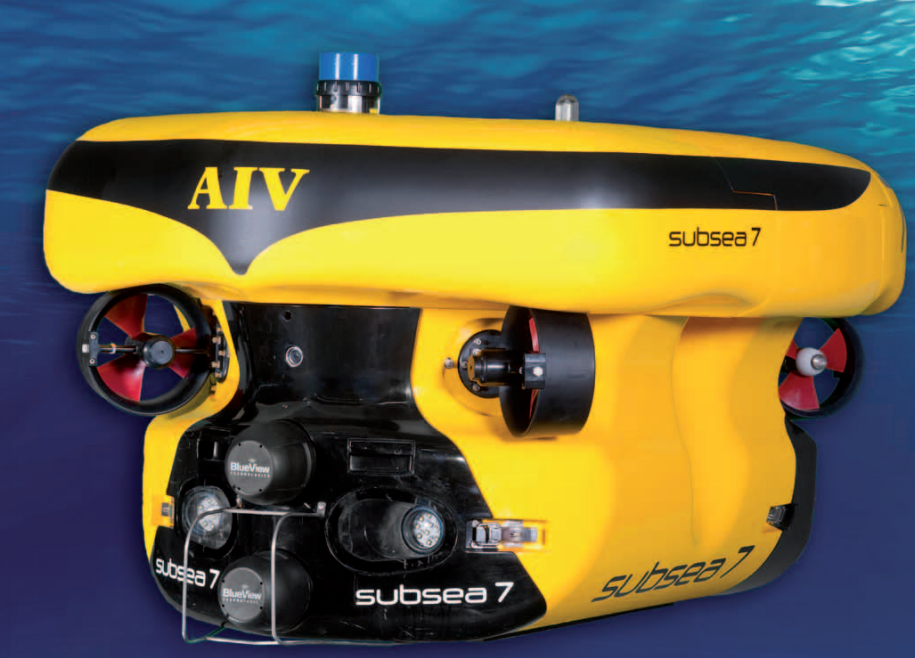
\includegraphics[width=0.48\textwidth]{subsea7AIV}
	\end{center}
	
	\caption{Subsea 7's AIV. This is the first commercial autonomous inspection vehicle for subsea operations \cite{pressAIV}}
	%\vspace{-20pt}
\end{wrapfigure}

Subsea maintenance is perhaps the field that have seen the greatest advancements in autonomous inspection and maintenance. As offshore installations are moved to the seabed, maintenance and inspection has become a significant challenge. This has resulted in a widespread use of \acp{ROV}. Recent developments in other fields, e.g. computer vision, human-robot collaboration and machine learning, has resulted in new \acp{AIV} and \acp{AUV} capable of performing inspection and simple maintenance tasks autonomously\cite{subseaAIV}\cite{Ridao2015227}. A driving factor behind the transition from \acp{ROV} to \acp{AUV} is cost reduction through increased offshore campaign efficiency.

\subsubsection{Disaster Response}

\begin{wrapfigure}{r}{0.5\textwidth}
	%\vspace{-20pt}
	\begin{center}
		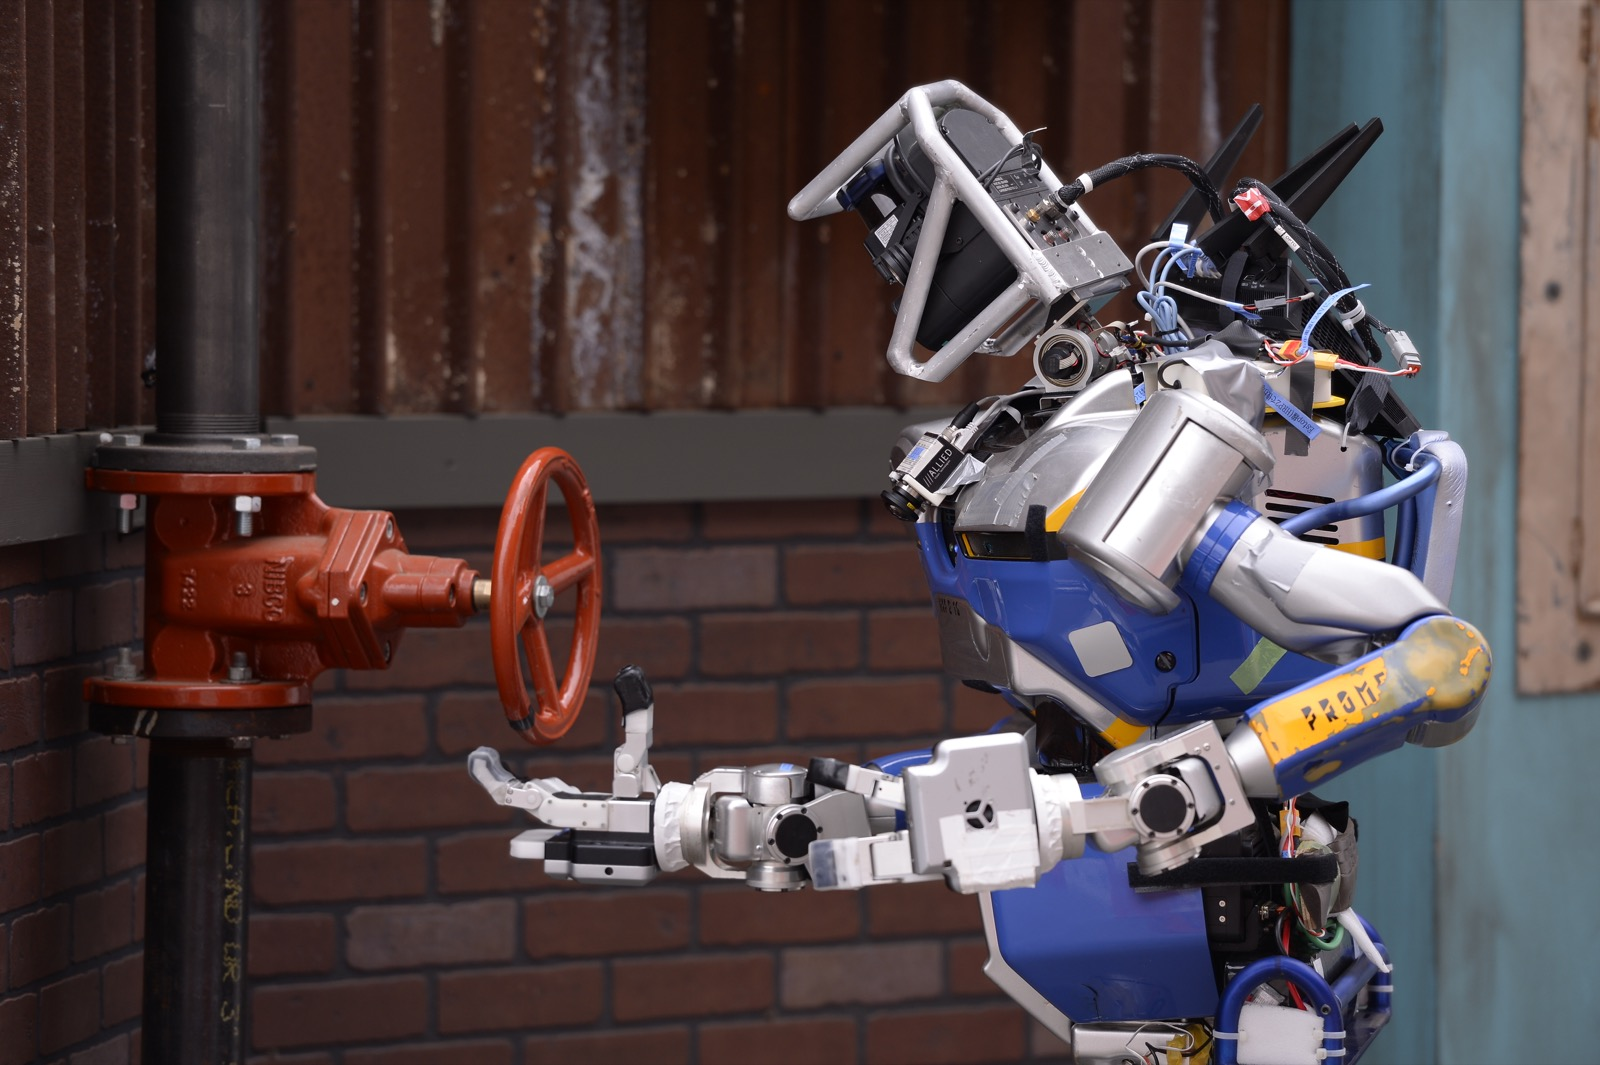
\includegraphics[width=0.48\textwidth]{HRP2_valve}
	\end{center}
	
	\caption{Team HRP2-Tokyo's robot turning a valve during DARPA Robotics Challenge 2015 (Image credits: DARPA Robotics Challenge)}
	%\vspace{-20pt}
\end{wrapfigure}

Robots in disaster response, relief and recovery solve many of the same problems faced by maintenance robots. Disasters, such as the tsunami which struck Japan in 2011, proved that much work needs to be done, both in terms of technical capabilities and logistical issues related to deployment and response times. The tsunami resulted in three core meltdowns at the Fukushima Daiichi Nuclear Power plant.

Many of the robots which were deployed at the Fukushima Power Plant were already ageing, and the operators had to receive training before deployment, thus increasing the response time\cite{doi:10.1108/01439911211249715}. A paper from Japan Atomic Energy Agency\cite{doi:10.1108/01439911211249715} highlights how the lack of stakeholder involvement could have been the cause of long response times. The same paper points out that the robots were developed for the sake of development, and not with emergency response as the main purpose\cite{doi:10.1108/01439911211249715}. 

\ac{DRC}\cite{DRC} was launched in response to the Fukushima disaster of 2011. The purpose of the competition is to accelerate innovation, research and development in robotics for disaster response in cases where humans cannot operate. Some of the tasks the competitors faces in 2015 include valve turning, traversing rubble and driving a vehicle through a course before egressing out of the vehicle.

\subsubsection{Topside Offshore and Onshore Robotic Maintenance}

\begin{wrapfigure}{l}{0.45\textwidth}
	%\vspace{-20pt}
	\begin{center}
		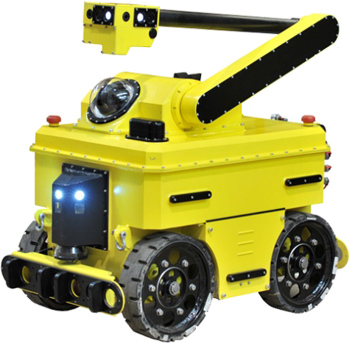
\includegraphics[width=0.42\textwidth]{sensabot}
	\end{center}
	
	\caption{An early version of the maintenance robot ''Sensabot'', developed by National Robotic Engineering Center (NREC) (Image credits: NREC)}
	\vspace{-20pt}
\end{wrapfigure} 

Today, autonomous and teleoperated inspection and maintenance is usually only found at subsea installations. Topside installations on the other hand are still maintained and inspected manually, with some notable exceptions. Small \acp{UAV} or \acp{RPAS} have become commonplace over the last decade. On topside installations, they are being used for visual inspection of inaccessible structural parts such as flare stacks or the exterior of oil rigs.

Some notable contributors to the field of robotic maintenance for \ac{OG} include ABB, \ac{Fraunhofer IPA}, Sintef ICT\cite{sintef_robot_consept} and NREC  at  Carnegie
Mellon University. 

NRECs contribution, Sensabot, is a remotely operated inspection robot designed for harsh and remote environments\cite{deploymentsensabot}. It is not designed to be autonomous, but rather as a tool to move personnel from hazardous environments to safe remote control rooms. Sensabot mark II will be certified for zone 1 explosive environments. This year (2016), the plan is to test the robot on site at the Kashagan field in Kazakhstan\cite{peerless2016robot}.

\ac{Fraunhofer IPA}\footnote{http://www.ipa.fraunhofer.de/en.html} has developed a robot, called \ac{MIMROex}. \ac{MIMROex} has capabilities which are quite similar to the prototype used during the work on this thesis. \ac{MIMROex} is equipped with a camera for visual inspections as well as microphones, vibration and sensors for fire and gas detection. It is also certifiable in accordance with the explosion protection standard IEC 60079\cite{MIMROex}. 

Both ABB and Sintef ICT has developed lab facilities to test various concepts for robotic maintenance. Both facilities use non-mobile robots which utilize a rich set of inspection and manipulation tools, as well as \ac{HMI} equipment for remote operation and control. The two research communities differ in that ABB has tested their solutions in real environments, which subjects their solution to ATEX requirements and an extensive risk management regime\cite{StepwiseApproachToRobotics}. 

Another effort towards robotic maintenance is the ARGOS challenge (Autonomous Robot for Gas and Oil Sites). The purpose of the challenge is to promote innovation, understanding and awareness towards robotic maintenance of \ac{OG} sites in harsh environments\cite{ARGOS}.

\section{Modelling and Simulation}

\subsection{Some Terminology}

\subsubsection{Coordinate Systems and Poses}

\subsubsection{Robot Joints}

All links are connected to each other by joints. 

Coordinate systems are essential in the field of robotics. 

\subsection{Robot Modelling}

\subsection{Simulating in Gazebo}

\section{ROS}

\subsection{Introduction}

The \ac{ROS} is a collection of software libraries, tools and drivers intended for robot software development. A \ac{ROS} installation can be tailored to meet the demands of a wide range of robots with varying complexity. \ac{ROS} is usually installed in the form of an already built Debian-package. These packages are only compatible with a few versions of Ubuntu which are specified on the \ac{ROS} homepage. When installed and configured, \ac{ROS} will run on top of Linux, and can be perceived as and extention of Linux itself. Installing \ac{ROS} from source is possible, but not recommended \cite{ROS_install}.

Roots of \ac{ROS} can be traced back to Stanford University at the beginning of the 2000s. At Stanford, several robotics software frameworks, including \ac{STAIR} and the \ac{PR} program, were created to provide dynamic, flexible and well tested foundations for further robot development and research. In 2007, a nearby start-up company and robot incubator, Willow Garage, sought to build upon these concepts, and initiated a collaborative and open development process of a new software framework. This framework eventually became \ac{ROS}\cite{ROS_history}\cite{rosbook15}. The framework can be used under the BSD open-source license\cite{BCD_license}. Today, \ac{ROS} comes in many forms and comprise hundreds of advanced packages, algorithms and drivers, making it applicable for hobbyists, industrial automation, research and everything in between. 

\subsection{Important ROS Concepts}
\label{sec:ros_concepts}
The following descriptions are included in order to provide a complete, self-contained description of the project implementation. Similar descriptions can be found on the official \ac{ROS} website\footnote{\url{http://www.ros.org/}}, as well as in any book on \ac{ROS} (for example \cite{rosbook15}). 

\subsubsection{The ROS Graph}

A \ac{ROS} system comprise a set of small programs that communicate with each other through messages. These programs become nodes in the \ac{ROS} graph. The nodes communicate with each other by publishing and subscribing to topics that form the edges of the graph. A topic must have the format of one of the specific data types provided by \ac{ROS}. For example, a node which receives temperature data from a thermometer, may publish the data as a topic on the \ac{ROS} system with the type \texttt{sensor\_msgs/Temperature}. There are many other data formats, e.g. velocity messages, \texttt{geometry\_msgs/Twist}; images, \texttt{sensor\_msgs/Image}; odometry messages, \texttt{nav\_msgs/Odometry} and so on. Each node in the graph are typically POSIX processes, and the edges are TCP connections\cite{rosbook15}. A minimal example of a graph is shown in figure \ref{fig:minimum_graph}.

\begin{figure}[p]
    \centering
    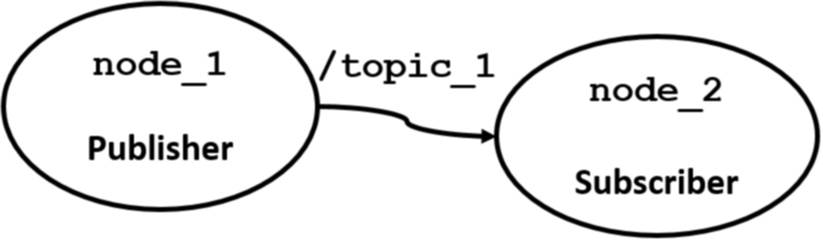
\includegraphics[width=0.8\textwidth]{minimum_graph_bl}
    \caption{A minimal \ac{ROS} graph. There are two nodes, \texttt{node\_1} and \texttt{node\_2}. \texttt{node\_1} publishes data, i.e. a topic, by the name \texttt{topic\_1}. \texttt{node\_2} can receive the data by subscribing to \texttt{topic\_1}.}
    \label{fig:minimum_graph}
\end{figure}

\subsubsection{roscore}

\texttt{roscore} is an essensial part of any \ac{ROS} system as it enables nodes to communicate with each other. An instance of \texttt{roscore} must be started before launching any nodes. When a node is started, it will inform \texttt{roscore} of which topics it publishes and which topics it wish to subscribe to. Then, \texttt{roscore} will provide the information which allows the node to form a peer-to-peer connection to other nodes.

\subsubsection{Project Structure and the \textit{catkin} Build System}

The source code in a \ac{ROS} system is organized into packages. Each package provides a specific functionality to the system. Some packages can be downloaded and installed from a remote repository, while other packages will be created by the in-house developers for their specific robotic system. In this project, locally created ROS-packages were placed into a \textit{catkin workspace}. This workspace contains the  original source code and build specifications. Details are provided in chapter \ref{chp:implementation}. As presented in\cite{ROS_tut_pkg}, a general workspace structure is as follows:

\begin{verbatim}
workspace_folder/        -- CATKIN WORKSPACE
  src/                   -- SOURCE SPACE
    CMakeLists.txt       -- 'Toplevel' CMake file, provided by catkin
    package_1/
      CMakeLists.txt     -- CMakeLists.txt file for package_1
      package.xml        -- Package manifest for package_1
    ...
    package_n/
      CMakeLists.txt     -- CMakeLists.txt file for package_n
      package.xml        -- Package manifest for package_n
\end{verbatim}

A \ac{ROS} project will usually utilize the catkin build system.

\subsubsection{\texttt{roslaunch}}

\texttt{roslaunch}\cite{ROS_launch} is a \ac{ROS} package tool used to launch multiple nodes from a single command line. This is useful for larger projects with many nodes, interactions and parameters. Exactly which nodes to launch is defined in XML-files with the \textit{.launch} extension. In a launch file, the developer can group nodes together, pass arguments to the nodes and launch other launch files. Launch files can be launched from the command line as follows:

\begin{verbatim}
$ roslaunch <package name> <launch file name>.launch <argument1>:=true
\end{verbatim}

\subsection{An Overview of ROS-Related Tools}

\subsubsection{Robot Modelling In URDF}

\ac{URDF} is an XML-like format for describing robots. The robot description is made up of links and joints. Each link description contains information of its shape, inertial tensor, collision boundaries. The links are connected to each other by joints.

\subsubsection{Visialization in \texttt{rviz}}

\texttt{rviz} is an invaluable tool for visualizing on-line robot behaviour. Simply put, \texttt{rviz} is created to visualize what the robot sees, and how it plans ahead. Many of the images in the following chapters are from \texttt{rviz}. 

\subsubsection{Simulation in Gazebo}


\subsection{Notable Robots Running ROS}

\paragraph{PR2 - Personal Robot 2}

PR2, developed by Willow Garage is one of the first robots designed to run \ac{ROS} \cite{rosbook15}, and also one of the most advanced and capable robots with \ac{ROS} today. PR2 is build for research and development of service robot applications. The navigation stack used in this thesis has been tested on the PR2. \cite{tbd} describes how the PR2 used the navigation stack to autonomously navigate 42 km (26.2 miles). The PR2 is available for sale at the price of \$280,000.00\footnote{https://www.willowgarage.com/pages/pr2/order}(2016).

\paragraph{TurtleBot} 

TurtleBot is a cheaper ROS-ready alternative to PR2. It is consists of a mobile base with differential drive, and a shelf system for mounting laptop computers and sensors.

\paragraph{Robonaut 2}

Robonaut 2\footnote{\ac{ROS} in space from ROSCon 2014: \url{https://vimeo.com/106993914}}, a dexterous humanoid robot, currently resides within the \ac{ISS} 400 km above the earth's surface. In 2014, a SpaceX Dracon capsule brought \ac{ROS} as well as a pair of legs for Robonaut up to the \ac{ISS}\cite{ROS_space}. Robonaut is designed for research on how robots can support the crew in maintaining and operating the space station. A potential application of Robonaut is to perform extra vehicular activities and other maintenance tasks, thus freeing up valuable time for the crew.

Being the first robot with \ac{ROS} to be launched into space, 

\paragraph{Industrial Hardware}

The ROS-industrial program\cite{ROS_industrial} provides hardware interfaces to various industrial equipment. An example is ABB's IRB-2400, where \ac{ROS}-industrial provides package for motion planning software (MoveIt!) and trajectory downloading\cite{ROS_industria_hardware}. 

\section{Software}

\subsection{Qt}

\subsection{PCL}

\section{The Kinect Sensor}

\section{Software Tools}

\subsection{Point Cloud Library}

\subsection{ROS}

\subsection{Qt}


\subsection{Current Research and Applications}

\section{Introduction to Sensors in Autonomous Robots}

\subsection{Depth Cameras}

\subsubsection{Different Methods for Depth Perception}

A depth camera can be described as a regular color video camera with the ability to create spatial images. In the context of this thesis, a depth camera can  more precisely be described as a RGB-D camera, where the letters RGB-D are short for red, green, blue and depth. In a regular RGB camera, a spatial scene will be projected onto a rectangular pixel grid where each pixel contains intensity values for red, green and blue colors. These pixel values represents the detected scene. A major problem with RGB cameras is the significant loss of information. The information loss is mostly a consequence of 3d to 2d projection and digital quantization. RGB-D cameras have the means to reduce this information loss by mapping the pixel values to spatial coordinates. The atomic parts in 3d images are usually represented as points in a point cloud or cubic volumes, also known as voxels.

Different variations of depth cameras will usually fall into one of two categories: active or passive. Passive sensors perceive the surroundings as it is, without actively interfering with the environment as a part of the sensing process. A typical passive RGB-D sensor is the stereo camera. Stereo cameras use a stream of synchronized image pairs to perceive depth. The image pairs are displaced along the horizontal axis, and the depth information is extracted by searching for mutual information in the image pairs. How far the information is displaced from the left to the right image is directly related to how far away from the camera the information source is located. 

Active sensors depend on some form of projection onto the surroundings. For depth cameras, the projection is usually in the form of laser or infra red light. In RGB-D cameras it is essential that the projected light is distinguishable from the visible spectrum. The Kinect sensor used in this project is an example of an active RGB-D sensor. A proper introduction to the Kinect will follow shortly.

\subsubsection{Natural User Interfaces - Origin of the Kinect}

The idea behind a \ac{NUI} is to make the \ac{HMI} as seamless and natural as possible. A \ac{NUI} allows the user to communicate without tools such as a keyboard or a mouse. For decades, \ac{NUI}s have only existed as ideas, science fiction or research projects. This has changed dramatically over the last ten years, and \ac{NUI}s can now be considered to be ubiquitous. Today, the most common form of \ac{NUI}s is the touch screen found in smart phones and tablets. 

The Microsoft Kinect sensor was initially designed as a \ac{NUI} for the Xbox 360 gaming console. The sensor allows users to use gestures and sounds to play console games. Later on, Microsoft has released SDKs, enabling developers to create \ac{NUI} applications for for Windows. 

\subsubsection{Kinect for Xbox 360}

Kinect for Xbox 360 is the RGB-D sensor used in this project. The device  was initially intended as a \ac{NUI} for gaming and office applications, and was the first consumer grade sensor to utilize structured light. Possible use cases were inspired by early \ac{NUI} research at \ac{MIT} and, later on, the science fiction movie Minority Report, where Tom Cruice interacts with a computer by using hand gestures \cite{kinect_book}. The Kinect sensor is equipped with a depth sensor, a regular color camera, a microphone array and a tilt motor(figure \ref{fig:kinect360_exp}). The color camera in combination with the depth sensor forms what is usually referred to as a RGB-D sensor, i.e. a combined color and depth camera (figure \ref{fig:kinect360_exp}). This feature, combined with the relaticely low cost and accessability of the sensor has contributed to make the Kinect very popular in research projects related to \ac{SLAM} and robotics. In the three first years since it's release in 2010, over 3000 papers in well-known journals and proceedings were devoted to research on the Kinect sensor. Roughly 500 of these papers focused on \ac{SLAM} or 3d reconstruction\cite{Berger2013}. Some of the other papers focused on some of the weaknesses with the sensor, such as detection of glass surfaces and having several sensors in the same area. 


Today, the the Kinect for Xbox 360 has been succeded by the Kinect for Xbox One, and is now considered to be a legacy device. Those considering to use the legacy Kinect should be aware of that it is becoming increasingly difficult, if not already impossible, to get hold of a new Kinect for Xbox 360. 

\begin{figure}[p]
    \centering
    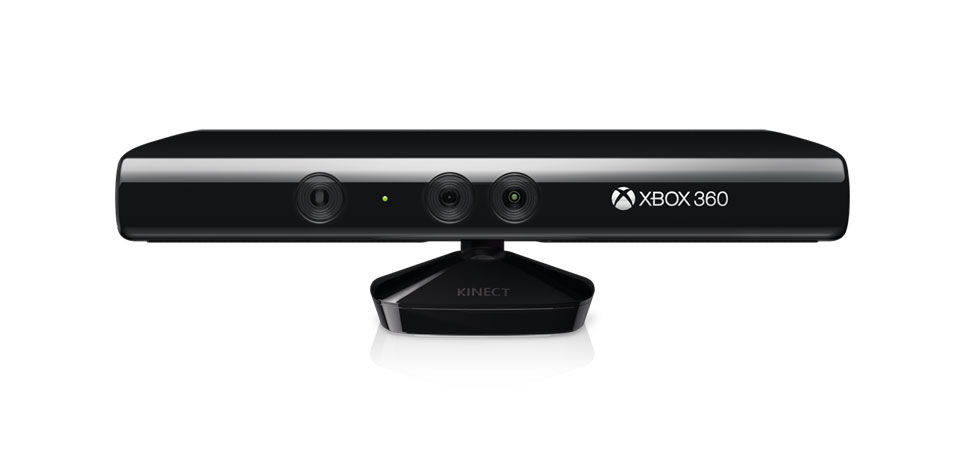
\includegraphics[width=0.8\textwidth]{kinect360}
    \caption{Awesome Image}
    \label{fig:kinect360}
\end{figure}

\begin{figure}[p]
    \centering
    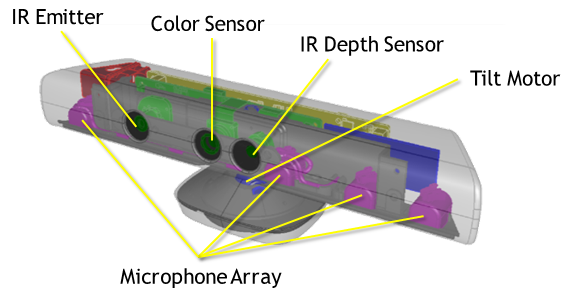
\includegraphics[width=0.8\textwidth]{kinect360_exp}
    \caption{Awesome Image}
    \label{fig:kinect360_exp}
\end{figure}


\subsection{Plannar Laser Sensors (LIDAR)}

A plannar laser sensor, known as e.g. laser proximity sensors or laser radars, can all be referred to as LIDARs. 

\subsubsection{Scanning Laser Range Finder, URG-04LX-UG01}


\subsection{Odometers}

\subsection{Sensor Fusion}


\section{Simultanious Localization and Mapping (SLAM)}

\subsection{Introdunction to SLAM}

\ac{SLAM}, also known as \ac{CLM}, is a class of solutions to the problem of determining an agents location and pose in an unknown environment, while simultaneously mapping the same environment.

\subsection{Hector SLAM}

\subsection{RTAB-Map}
\label{sec:RTAB-Map}

\ac{RTAB-Map} is developed by IntRoLab at Université de Sherbrooke in Canada. It is a \ac{SLAM} system developed for long term operations in large environments. The system is also intended to handle the ''kidnapped robot-problem'', i.e. multi-session mapping. This is useful whenever the robot is shut down and moved to an unmapped part of the same area, where it will start a new mapping session. \ac{RTAB-Map} is the core feature that has been integrated into the robot described in this thesis. Some factors which motivated the use of \ac{RTAB-Map} are:

\begin{itemize}
	\item It is a \ac{SLAM} method which requires an RGB-D sensor, for example a Kinect. The problem description for this project requires a vision based solution.
	\item \ac{RTAB-Map} has a \ac{ROS} wrapper, \texttt{rtabmap\_ros}, which eases the process of integrating it with the mobile robot.
	\item It includes 3d obstacle detection.
	\item It has a memory management system intended for large scale multi-session mapping.
	\item \ac{RTAB-Map} can be used for object detection. This can be done by linking \ac{RTAB-Map} to OpenCV and the non-free feature detectors \ac{SIFT} and \ac{SURF}.
\end{itemize}

The source code and \ac{ROS} wrapper is currently maintained, and new features and bug-fixes are added regularly. \ac{RTAB-Map} has two distinctive solutions to the \ac{SLAM} problem: Visual loop closure detection and a memory management system for large data sets. The following paragraphs provides an overview of how \ac{RTAB-Map} works. Detailed descriptions of the loop closure detection and memory management approach is provided in  \cite{labbe13appearance}, while the \ac{SLAM} method is presented in \cite{labbe14online}. Further details can be found on the project's Github page\footnote{\url{http://introlab.github.io/rtabmap/}}.

\subsubsection{Graph Based Mapping}

\ac{RTAB-Map} uses a graph structure with nodes and edges to represent the map. New nodes are continuously added to the systems working memory as time passes. In this method, the graph edges are referred to as \textit{links}. There are two types of links: neighbour links and loop closure links. Each node is a location in the map, and the links contain geometrical transformations between the node locations. Figure \ref{fig:rtabmap_graph} illustrated the graph concept.

\begin{figure}[p]
    \centering
    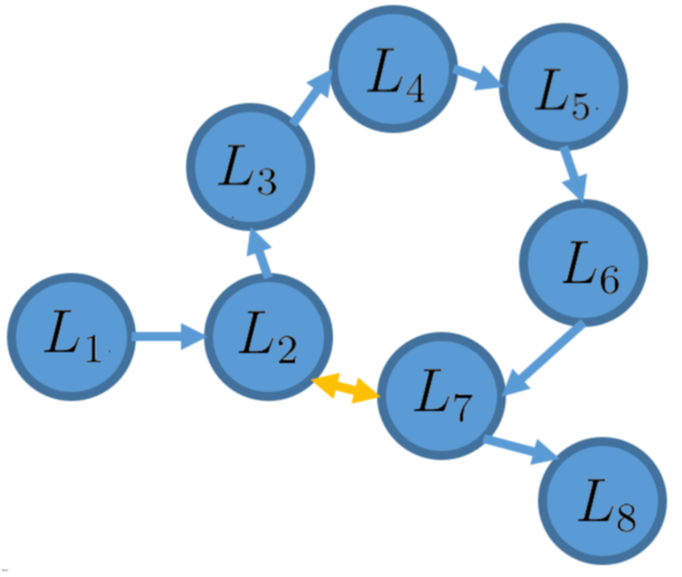
\includegraphics[width=0.5\textwidth]{rtabmap_graph_bl}
    \caption{Conceptual illustration of a graph created by \ac{RTAB-Map} over time $1 \leq t \leq 8 $. A loop closure hypothesis was accepted at $t=7$, as shown by the yellow arrow. Feature descriptors in $L_2$ and $L_7$ are sufficiently similar to accept this as a loop closure.}
    \label{fig:rtabmap_graph}
\end{figure}

\subsubsection{On-line Mapping of Large Environments}



\subsection{RGBD SLAM and Octomap}

Octomap\cite{hornung13auro} is another 3d mapping framework available for \ac{ROS}. Similar to \ac{RTAB-Map}, Octomap can also be used as a standalone version. 

Maps are represented by memory efficient Octrees where each leaf node represents a cube, or voxel, in the volumetric map. The voxel can be either occupied, free or unexplored. The volume of the cube is determined by how deep in the tree the leaf node is located. In a \ac{ROS} graph, the Octomapping is performed by the node \textit{octomap\_server}. This node  will subscribe to point cloud messages \texttt{sensor\_msgs/PointCloud2}, and return volumetric occupancy maps, i.e. Octomaps.

There are several approaches to \ac{SLAM}  which uses Octomaps. An example that stands out in the context of \ac{ROS} is\cite{endres20143}; a \ac{SLAM} approach which depends on a RGB-D sensor, and relies on Octomap for efficient map storage.

This mapping framework was not used in this project in order to limit the project scope, and because the alternative \ac{RTAB-Map} was associated with less uncertainty.

\section{Navigation}

\ac{ROS} has a built in navigation stack for 2d navigation. 
